$ A=a_3a_2a_1a_0, B=b_3b_2b_1b_0 $\\
$A,B\in [-8,7] $ بنابراین برای نمایش A و B در سیستم مکمل ۲ به ۴ بیت نیاز داریم.\\
$X=A-B \in [-15, 15]$ به ۵ بیت نیاز است\\
$|X|=|A-B| \in [0, 15]$ به ۵ بیت نیاز داریم\\
اگر $x_4=1 \rightarrow X < 0 $ بنابر این محاسبه می‌شود: $0-X$\\
اگر $x_4=0 \rightarrow X \ge 0 $ بنابر این محاسبه می‌شود: $0+X$\\
$R=|A-B| \in [0,15]$ به ۵ بیت نیاز است.


\begin{figure}[h]
	\centering
	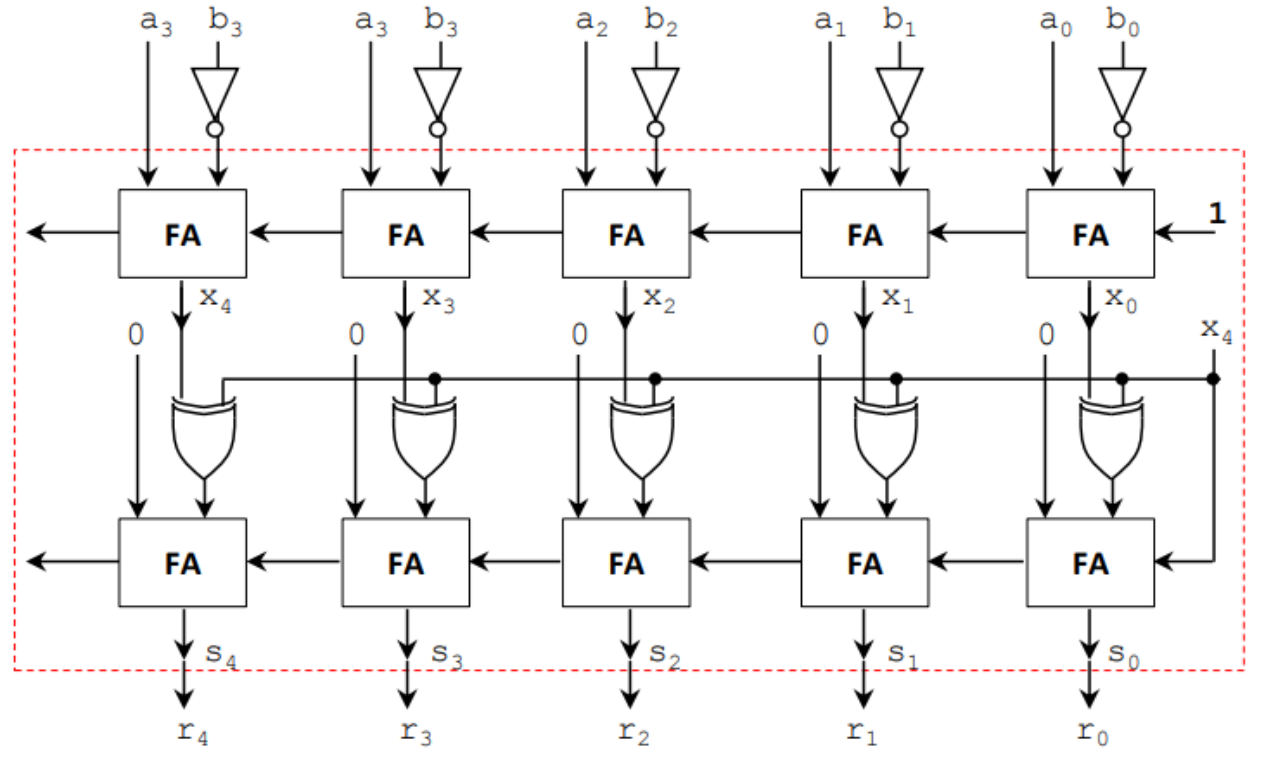
\includegraphics[width=0.8\textwidth]{fig/Q5.png}
	\caption{مدار طراحی شده برای سوال ۵}
	\label{Q5_Design}
\end{figure}